\documentclass[11pt]{article}
\usepackage[T1]{fontenc}
\usepackage{lmodern}
\usepackage[margin=0.85in]{geometry}
\usepackage{amsmath,amssymb,graphicx,booktabs,longtable}
\usepackage[round,authoryear]{natbib}
\usepackage[colorlinks=true,citecolor=blue,urlcolor=blue,linkcolor=blue]{hyperref}
\usepackage{microtype}
\graphicspath{{../reports/stage10/figures/}}
% Generated from results/stage10/summary.json. Do not edit.
\newcommand{\RudyCadences}{430387}
\newcommand{\RudyBaseline}{488.18}
\newcommand{\RudyDuty}{0.600}
\newcommand{\RudyNumax}{2233.60}
\newcommand{\RudyDnu}{103.3637}
\newcommand{\RudyCentroid}{2105.25}
\newcommand{\TutorialNumax}{2145}
\newcommand{\TutorialDnu}{103.1121}
\newcommand{\RudyAliasSpacing}{217.06}
\newcommand{\RudyAlias}{double}
\newcommand{\NullMeanRatio}{1.002}
\newcommand{\TessCandidateSectors}{15}

\newcommand{\numax}{\nu_{\max}}
\newcommand{\dnu}{\Delta\nu}
\setlength{\parskip}{0.35em}
\setlength{\parindent}{1em}
\pdfinfoomitdate=1
\pdftrailerid{}
\title{Topological organization of a stochastic stellar oscillation spectrum:\\
an auditable Kepler--TESS case study of KIC 10963065}
\author{Gabriel Wendell\\\small TopoAstero project}
\date{Paper I internal review freeze, 1 October 2026\\
\small Version 0.11.0; independent reproduction and claim review pending}
\begin{document}
\maketitle
\begin{abstract}
We present a reproducible, failure-aware benchmark of spectral persistence and
cylindrical echelle geometry for the solar-like oscillator KIC 10963065 (Rudy).
Twenty-one checksum-verified public Kepler and TESS products anchor a complete
observation capsule. The original Lightkurve tutorial gives
$\numax=\TutorialNumax\,\mu{\rm Hz}$ and
$\dnu=\TutorialDnu\,\mu{\rm Hz}$; a distinct Harvey-whitened envelope and ACF
pipeline gives $\RudyNumax$ and $\RudyDnu\,\mu{\rm Hz}$.
Localized finite path $H_0$ lifetimes equal elder-rule peak prominence exactly.
Their weighted location, $\RudyCentroid\,\mu{\rm Hz}$, is retained as a diagnostic,
not a calibrated replacement for the classical envelope. We report window-matched
conditional background tests, alias alternatives, 72 registered sensitivity
diagnostics, monthly resampling and stochastic realization scatter.
Cylindrical paths remain unidentified and do not establish estimator utility or
new frequency-ratio measurements. Delay topology is omitted under an earlier
registered negative decision. A 396-cell same-star degradation experiment uses
all eleven real TESS sector windows; actual TESS candidates remain unconfirmed.
The result is an auditable single-star case study with bounded claims, not
population validation or evidence of new information beyond classical controls.
\end{abstract}

\section{Introduction}
Solar-like oscillations are stochastic: the spectrum depends on mode excitation,
damping, finite observing duration, cadence integration and the spectral window.
The usual global observables $\numax$ and $\dnu$ summarize an oscillation envelope
and a nearly regular acoustic-mode comb. Echelle diagrams organize the comb and
expose degree-dependent ridges. Their interpretation is inseparable from quality
masks, background models and the distinction between one realization and a
population of stars \citep{Lund2017,SilvaAguirre2017}.

Persistent homology tracks connected components and loops through a filtration.
Applied to a one-dimensional superlevel spectrum, it provides localized births
and merger saddles. This can be a compact organization of spectral peaks, but it
does not by itself establish additional physical information or estimator accuracy.
Known diagram-stability results concern perturbations of a fixed field and complex,
not the correctness of a spacing selected from a collection of folds
\citep{CohenSteiner2007}. A cylindrical echelle additionally requires a periodic
phase boundary: the left and right display edges represent the same phase.

TopoAstero's development sequence separated analytic validation, stochastic
simulations, classical controls and mathematical audits before this case study.
The delay branch failed its registered simulation tests and was dropped. The
cylindrical branch passed geometry tests but failed estimator-utility and interval
coverage gates; its scientific scope remains geometry only. The present paper
therefore asks whether a fully auditable observation pipeline can connect these
constructions to a real star while preserving their demonstrated limits.
Rudy was already the descriptive benchmark in the classical pipeline. It is not
an untouched confirmation star, and this study does not open population or final
holdout partitions.

\section{Observations and locked analysis capsule}
\subsection{Public products and provenance}
The Kepler short-cadence benchmark comprises ten tutorial products across Q2,
Q5, Q6 and Q7. The primary finite, quality-filtered series retains
\RudyCadences\ cadences over an absolute span of \RudyBaseline\ days with
cadence-mask duty \RudyDuty. Eleven homogeneous SPOC two-minute TESS light curves
cover sectors 14, 15, 40, 41, 53, 55, 74, 75, 80, 81 and 82 for TIC 48450369.
Every product is identified by a frozen MAST URI, payload SHA256 and size; the
capsule records flux, quality, time system, BJD reference, cadence and exposure
metadata. A missing or changed payload stops execution rather than replacing
the registered bytes. The official tutorial supplies the classical reproduction
context \citep{LightkurveTutorial,Lightkurve2018,MAST2026}.

\subsection{Preprocessing roles}
PP-01 uses PDCSAP flux and the Lightkurve default Kepler quality mask, with only
mission detrending and per-month normalization. PP-02 uses quality equal to zero
and five-sigma clipping. PP-03 uses SAP flux, the default mask, five-sigma clipping
and a 1001-cadence Savitzky--Golay high-pass. PP-04 uses the hardest quality mask
and five-sigma clipping. PP-05 supplies analytic FFT/unit tests; PP-06 applies the
default TESS quality mask to individual SPOC sectors. Nonfinite flux is removed
before inference. Absolute timestamps and gaps are preserved. Integer quality
masks and per-product cadence counts are recorded from the locked installation.
No branch is chosen using a topological score.

The Stage 10 configuration was locked before its new topology and null results.
This is an implementation lock, not an externally timestamped preregistration.
Earlier Stage 3 descriptive Rudy results were already known. This distinction is
part of the claim ledger and prevents the present results from being presented
as an independent discovery.

\section{Methods}
\subsection{Classical spectrum and background}
We reproduce the Lightkurve PSD, default log-median flattening, ACF2D global
parameters and uncorrected scaling quantities separately from the independent
Harvey/ACF pipeline. The latter evaluates a one-sided Lomb--Scargle PSD from
100 to 8000 $\mu{\rm Hz}$ in ppm$^2/\mu{\rm Hz}$, comparing zero-, one- and
two-component rational Harvey continua with exponent four. The interval
1500--2800 $\mu{\rm Hz}$ is excluded from background fitting. Minimum BIC chooses
the primary continuum; all families remain in the sensitivity table.
Because windowed ordinates can be correlated, BIC is a descriptive ranking,
not a posterior probability.

Native ordinates are mean-rebinned to 0.2-$\mu{\rm Hz}$ centers for the reduced
spectrum. When a diagnostic output grid is finer than a segment's native
resolution, interpolation is confined to supported frequencies and is explicitly
not counted as additional information. The primary classical envelope maximizes
a 35-$\mu{\rm Hz}$ Gaussian-smoothed $P/B$ in 1700--2500 $\mu{\rm Hz}$.
The spacing estimator uses a 0.5-$\mu{\rm Hz}$ smoothed whitened spectrum in a
275-$\mu{\rm Hz}$ half-width, with an ACF search around the classical scaling
prediction. This is a distinct estimator from the tutorial. PSD units and FFT
endpoint conventions are independently tested \citep{VanderPlas2018,Astropy2022}.

\subsection{Localized spectral persistence and alias controls}
The primary filtration is exact superlevel path $H_0$ on
$f(\nu)=\log[P(\nu)/B(\nu)]$, after 1-$\mu{\rm Hz}$ smoothing of power.
For a finite component born at a peak and merged at a saddle,
$\pi=f_{\rm birth}-f_{\rm merge}$. The elder rule makes $\pi$ exactly the
corresponding elder-rule prominence; an independent implementation checks the
identity on the observation. Essential components retain localization but have
no finite lifetime and are excluded from numerical summaries.
Ratio, residual and a z-score using a registered 10\% background allowance are
mandatory alternative normalizations; the allowance is not a fitted posterior.

The persistence-weighted centroid in 1700--2500 $\mu{\rm Hz}$ is compared with
the classical envelope. A pair-difference/autocorrelation comb diagnostic scans
57 spacings from 20 to 300 $\mu{\rm Hz}$. ACF and power-spectrum-of-power-spectrum
(PSPS) controls use the same supported spectrum. Boundary winners, half/double
alternatives and disagreement are retained. Neither the centroid nor the broad
comb maximum is automatically interpreted as a calibrated seismic estimate.

\subsection{Periodic echelle geometry}
We fold the log-ratio spectrum to a 24-phase-bin finite cylinder, with phase
periodic and the row direction finite. Orders lacking 75\% phase support
contribute no vertices. The frozen Stage 8 score combines normalized finite
$H_0$ persistence and a topology-free circular ridge graph:
\[
S_{\rm cyl}=0.55\,S_{H_0}+0.45\,S_{\rm graph}.
\]
The registered classical ACF anchor determines half, nominal and double families,
each evaluated at relative spacings 0.90, 0.95, 1.00, 1.05 and 1.10.
The published spacing is never an anchor for score selection. Each null
realization repeats the classical-anchor policy. Graph, conventional folded-profile
contrast, Hough, ACF and PSPS controls accompany the topology.

A periodic loop can encode the geometry of the domain without establishing a
stellar ridge identity. The competing graph paths have no defensible angular-degree
anchor. Accordingly we report no inferred $r_{02}$, $r_{01}$ or $r_{10}$.
Ratios computed from externally identified published modes are formula audits,
not topological measurements. The new conditional ridge proposition from Stage 9
is still awaiting independent proof review and is excluded from headline claims.

\subsection{Conditional nulls and finite Monte Carlo precision}
We draw 256 stationary Gaussian background realizations from the selected Harvey
continuum on a full Kepler cadence grid spanning the real absolute times.
The generative density is corrected by measured sampling duty to reconcile the
full-span LS density with retained-exposure white-noise variance. Draws are
corrected for the analytic mean two-tap linear-interpolation power response,
interpolated to the observed barycentric timestamps and processed through the
same native LS frequency policy, rebinning and smoothing.
This discretization approximates the finite sampling operator; the ensemble
mean whitened power, \NullMeanRatio, is retained as a nuisance-model diagnostic.

For each statistic family we retain the maximum over its registered
frequency/spacing search, giving
\[
p={1+\#\{S^{(b)}_{\max}\geq S_{\rm obs}\}\over 257}.
\]
Upper-tail ties are counted conservatively. Wilson intervals describe the
underlying simulated exceedance probability; MC standard errors and counts are
reported. Holm correction controls the seven reported families within this
conditional model. The minimum attainable unadjusted $p$ is $1/257$.
The fit is not reestimated in each draw, and the test does not calibrate
background-fit uncertainty, instrumental residuals or nonlinear detrending.
No raw-bin Gamma bound is applied to a smoothed or selected score.

\subsection{Uncertainty and stellar scaling}
Quarters and cumulative absolute baselines are analyzed with the full-span
background held fixed, after converting each segment PSD by segment duty divided
by full-span duty to the same density convention. Cumulative points overlap. Ten nonoverlapping monthly
PSDs receive the same duty conversion, are resampled 256 times and averaged by retained cadence count. These
intervals target the monthly-averaged-spectrum estimator, which differs from the
coherent full-span periodogram. Sixty-four Gaussian draws of a smoothed observed
PSD describe conditional stochastic repeat scatter. Sixty-four monthly
cylindrical resamples provide alias diagnostics only, because coverage failed
the earlier simulation gate.

We retain these components alongside the range across all 72 registered branch
diagnostics. They are not combined as independent errors. Uncorrected scaling
calculus uses $T_{\rm eff}=6140\pm77$ K and
$M\propto\numax^3\dnu^{-4}T_{\rm eff}^{3/2}$,
$R\propto\numax\dnu^{-2}T_{\rm eff}^{1/2}$ and
$g\propto\numax T_{\rm eff}^{1/2}$.
Draws preserve paired seismic bootstrap values and separate temperature variation.
Composition, structural corrections and solar-reference systematics remain
unquantified. The scaling outputs are conditional diagnostics, not a physical
stellar posterior \citep{Viani2017,SilvaAguirre2017}.

\subsection{Kepler-to-TESS degradation}
We integrate the piecewise-linear Q5 Kepler curve through ideal 120-second
boxcar exposures at source offsets 0, 30 and 60 days. Exposures crossing source
gaps longer than 180 seconds are rejected. The experiment applies all eleven
actual TESS retained-timestamp windows, duration cuts of 13.7 and 27.4 days,
additional retention fractions 1 and 0.8, and added-noise variance factors
0, 1 and 2. Additional white noise matches the positive difference between
the actual TESS and degraded Kepler high-frequency noise floors; existing
Kepler noise is never subtracted.

The 396 cells record actual duration, duty and source-coverage loss. They reuse
correlated source realizations and do not represent independent stars.
Actual sectors are evaluated separately using the earlier fixed feasibility
rule (envelope SNR at least 1.20, reference-conditioned envelope/spacing
agreement and ACF peak at least 0.08). The native 1500--2700-$\mu$Hz sidebands,
1800--2500-$\mu$Hz search and primary tutorial reference values exactly preserve
the Stage 3 feasibility policy. This rule yields marginal candidates,
not blind detections or confirmations. The ideal boxcar cannot match TESS
bandpass, detector systematics, detailed exposure dead time or nonlinear
cotrending.

\section{Simulation evidence and inherited decisions}
The registered Stage 4 simulation design spans observing duration, cadence,
duty, noise, mode lifetime, visible orders, background mismatch and alias
conditions. Stage 6 showed exact prominence equivalence and supported an
equivalence-limited spectral claim, with explicit null and classical controls.
The Stage 7 evaluation yielded zero BH rejections for both phase-randomized and
IAAFT-surrogate paths and no positive held-out predictive increment; delay PH
was dropped from the critical path.

Stage 8 had only five detectable evaluation cells. Correct-alias accuracy was
0.20 for the cylindrical score and 0.60 for the graph control; nominal
90\% interval coverage was 0.20. Thus geometry passed and estimator utility
did not. These are small simulation-gate summaries, not population estimates.
The current Rudy result cannot reverse them merely by agreeing with a published
spacing. Figure~\ref{fig:placement} locates the observations against the simulation
coordinates without treating the comparison as inverse calibration.

\section{Rudy results and ablations}
\subsection{Classical baseline and spectral organization}
The tutorial is reproduced at $\TutorialNumax$ and $\TutorialDnu\,\mu{\rm Hz}$.
The independent primary envelope and spacing are $\RudyNumax$ and
$\RudyDnu\,\mu{\rm Hz}$. Differences reflect pipeline conventions and finite
realization behavior, rather than a correction forced to a reference.
The published LEGACY context is
$\numax=2203.7^{+6.7}_{-6.3}\,\mu{\rm Hz}$ and
$\dnu=103.179\pm0.027\,\mu{\rm Hz}$ \citep{Lund2017}.
Published-mode overlays inspect local spectral consistency; selecting a peak
near an externally supplied frequency is not blind peak bagging.
Table~\ref{tab:branches} retains all preprocessing branches.

The primary persistence centroid is $\RudyCentroid\,\mu{\rm Hz}$, displaced
from the classical envelope. Finite lifetimes reproduce prominence to numerical
precision. This provides localized organization without establishing a new
signal-strength observable. The broad comb diagnostic has a boundary maximum
and competing aliases, while ACF/PSPS alternatives differ. The cylinder's
largest registered score occurs in the \RudyAlias\ family at
$\RudyAliasSpacing\,\mu{\rm Hz}$. We retain that choice and all competing trials
as a diagnostic rather than declaring a new spacing measurement.

\subsection{Conditional tests and sensitivity}
Table~\ref{tab:nulls} gives all seven maximum-statistic tails and Holm-adjusted
values. Rejection, where present, is evidence against the fitted conditional
background-only model. It does not demonstrate topology's incremental utility
relative to the graph, ACF, PSPS or prominence controls.
The 48 preprocessing--background--normalization combinations and 24 one-factor
background-scale, smoothing and resolution diagnostics remain visible.
Background families can change envelope contrast and centroid interpretation
even when a classical comb spacing is comparatively stable. No favorable branch
is selected after examining the score.

Table~\ref{tab:uncertainty} separates the monthly estimator, full-span point,
monthly bootstrap interval and pipeline range. Quarter and cumulative diagnostics
show observed window/realization dependence. Conditional stochastic scatter and
seismic/temperature scaling tables are supplied separately. Pipeline ranges and
realization scatter are not independent stellar error budgets.

\subsection{Transfer results}
The degraded Kepler series is evaluated through every registered real TESS
window, and actual sectors occupy the same noise/duration context. Under the
fixed primary feasibility policy, marginal actual-sector candidates occur in
sectors \TessCandidateSectors. They remain unconfirmed. The empirical conditional
fractions in Figure~\ref{fig:transfer} describe the reused Q5 experiment, not a
binomial rate for independent realizations or a population detectability law.

\begin{table}[htbp]\centering\small
\caption{Mandatory preprocessing branches. The tutorial and independent estimators use different whitening and envelope conventions. All frequencies are in $\mu$Hz.}
\begin{tabular}{lrrrrr}\toprule
Branch & Cadences & Tutorial $\nu_{\max}$ & Tutorial $\Delta\nu$ & Classical $\nu_{\max}$ & Classical $\Delta\nu$\\\midrule
PP-01 & 430387 & 2145 & 103.1121 & 2233.6 & 103.3637\\
PP-02 & 363690 & 2175 & 102.9461 & 2152.8 & 103.2427\\
PP-03 & 430158 & 2175 & 102.5431 & 2152.2 & 103.2803\\
PP-04 & 363690 & 2175 & 102.9461 & 2152.8 & 103.2427\\
\bottomrule\end{tabular}\label{tab:branches}\end{table}
\begin{table}[htbp]\centering\small
\caption{Conditional fitted-background maximum-statistic tests. MC uncertainty and exceedance counts are provided in the machine-readable table. Holm controls the seven reported families within this conditional model.}
\begin{tabular}{lrrr}\toprule
Statistic family & Observed & Plus-one $p$ & Holm $p$\\\midrule
Smoothed envelope & 1.4326 & 0.0039 & 0.0272\\
Largest finite peak lifetime & 2.1213 & 0.0039 & 0.0272\\
Persistence comb maximum & 0.0757 & 0.0039 & 0.0272\\
Cylindrical combined maximum & 0.3893 & 0.0039 & 0.0272\\
Ridge graph maximum & 0.5861 & 0.0039 & 0.0272\\
ACF maximum & 0.6781 & 0.0039 & 0.0272\\
PSPS maximum & 0.0537 & 0.0039 & 0.0272\\
\bottomrule\end{tabular}\label{tab:nulls}\end{table}
\begin{table}[htbp]\centering\small
\caption{Distinct uncertainty targets. Bootstrap endpoints target the monthly averaged spectrum. The full-span point is a different estimator. Pipeline ranges include all 72 registered diagnostics; components are not combined.}
\begin{tabular}{lrrrr}\toprule
Quantity ($\mu$Hz) & Full span & Monthly point & Monthly bootstrap 95\% & Pipeline range\\\midrule
Classical envelope & 2233.60 & 2232.60 & [2142.10, 2435.70] & [2146.40, 2236.30]\\
Classical spacing & 103.36 & 103.42 & [102.89, 103.57] & [103.23, 103.37]\\
Persistence centroid & 2105.25 & 2098.05 & [2087.14, 2112.25] & [2092.48, 2125.69]\\
\bottomrule\end{tabular}\label{tab:uncertainty}\end{table}


\section{Discussion and limitations}
The useful deliverable is a fully inspectable connection between observations,
classical diagnostics, localized persistence, periodic geometry and failure
reasons. Known path-prominence equivalence prevents a novelty claim based solely
on peak lifetime. A periodic complex avoids a geometric seam artifact, but a
correct domain topology does not validate an estimator or assign degree labels.
The previous simulation failures remain part of the result.

The reference star was already inspected; nulls condition on a fitted stationary
continuum; Gaussian predictive draws do not reconstruct the complete excitation
and damping physics; quarter and source-window experiments share data.
Background-fit uncertainty, nonstationary instrument effects and stellar scaling
corrections remain outside the calibrated model. The finite null ensemble cannot
support extremely small false-alarm probabilities. Topological ratios and
population-level conclusions are withheld. The accompanying limitation register
records these restrictions claim by claim.

Independent human proof review of the new Stage 9 proposition and independent
Stage 10 reproduction/claim review remain pending. The current artifact is a
complete internal review draft and code freeze. Automated clean-process
reproduction is recorded separately; it is not an independent scientist's
attestation. This distinction protects the manuscript from overstating either
scientific validation or publication status.

\section{Data, code and reproducibility availability}
TopoAstero 0.11.0 supplies the frozen public identifiers, hash-verified acquisition
workflow, locked Python environment, configuration, per-cadence-count provenance,
all numerical tables, eight-claim ledger and ten PDF/SVG/PNG figure sets.
Raw public FITS files are reacquired into an external cache and are not bundled.
The command documented in the repository,
\texttt{uv run python workflows/reproduce\_stage10.py}, with a cache argument
and \texttt{--download}, regenerates the analysis and draft from public identifiers.
A fresh source copy, locked environment and new process check numeric tables and
headline outputs. Reduced-table replay is available for offline CI and is labeled
separately from raw-product reproduction.

The archive includes this editable LaTeX source, generated tables, checked
bibliography and compiled draft. No public code repository, journal submission,
Zenodo deposition or DOI is represented as completed. Those publication identifiers
must be supplied by the authors after the corresponding external actions.
The internal snapshot lists exact file hashes and the pending independent
review record.

\section{Conclusions}
Rudy connects a reproducible classical baseline to localized spectral persistence
and a correctly periodic echelle construction. The spectral representation
reorganizes known prominence information; cylindrical scores and unidentified
ridges remain geometry diagnostics under the inherited gate. Explicit null
scope, aliases, branch sensitivity and distinct uncertainty estimands narrow
the admissible claims. The Kepler--TESS experiment demonstrates a reproducible
same-star transfer protocol, with actual TESS observations retained as context.
No new degree-blind ratios, calibrated topological stellar parameters or
population generalization follows from this case study.

\clearpage
\appendix
\section{Journal figure suite}
Every figure uses TopoAstero's unmodified academic style TA-PLOT-1.0 and lists
its source tables in the machine-readable figure manifest.
\begin{figure}[p]\centering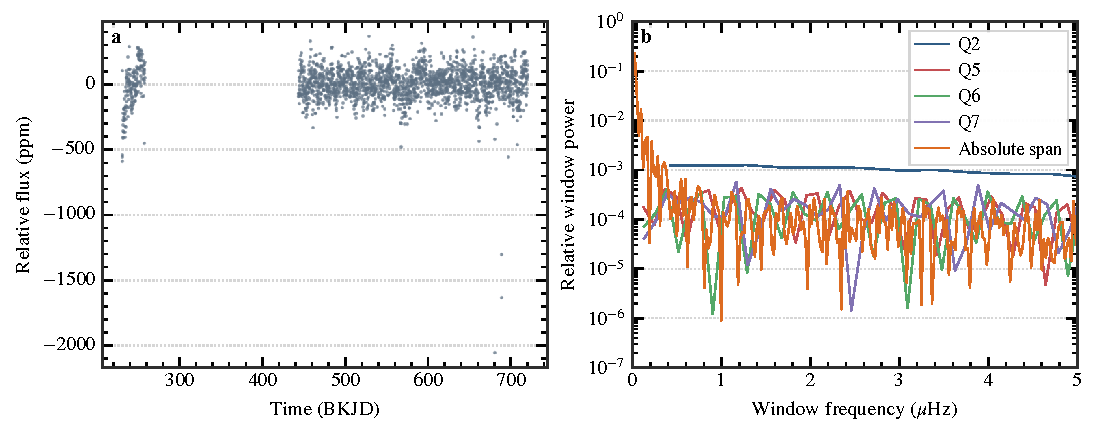
\includegraphics[width=\textwidth]{01_observation_window.pdf}
\caption{Absolute-time Kepler observations (every 200th cadence for display) and
cadence-mask windows. Inter-quarter gaps are retained.}\label{fig:window}\end{figure}
\begin{figure}[p]\centering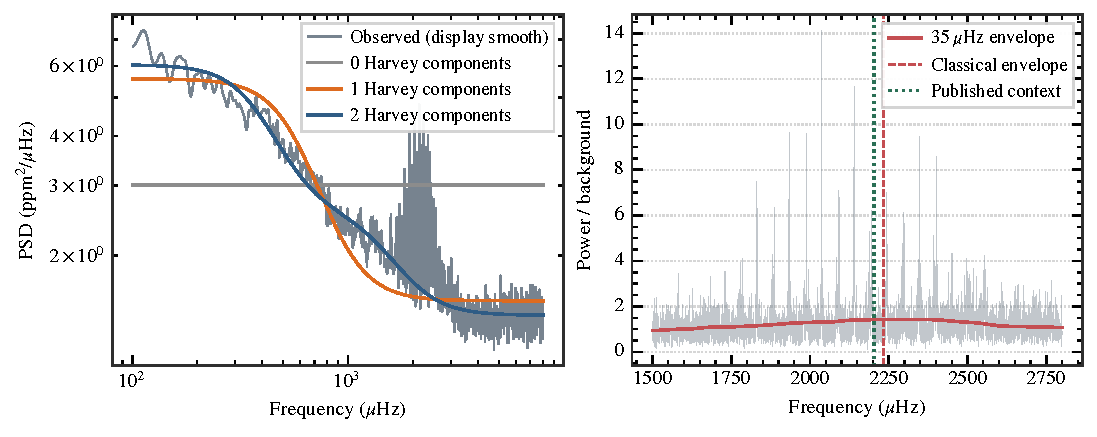
\includegraphics[width=\textwidth]{02_psd_background.pdf}
\caption{PSD, all registered background families, and the independently
estimated envelope. The published context is not a tuning target.}\end{figure}
\begin{figure}[p]\centering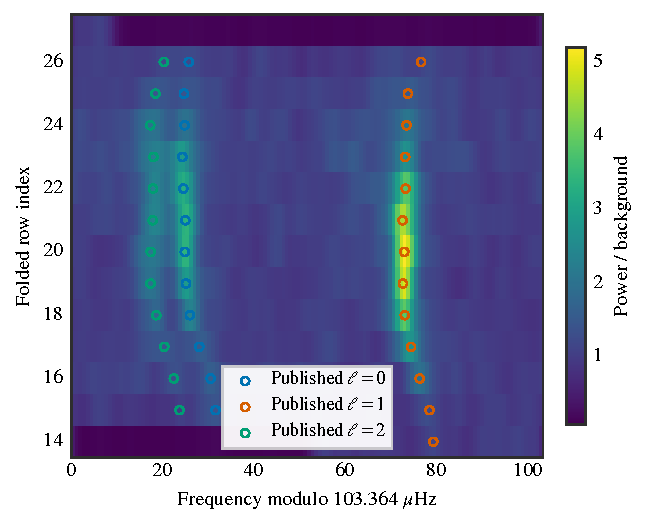
\includegraphics[width=0.72\textwidth]{03_ordinary_echelle.pdf}
\caption{Ordinary echelle at the classical ACF spacing, with external
degree-identified modes. Folded rows are not physical radial-order labels.}\end{figure}
\begin{figure}[p]\centering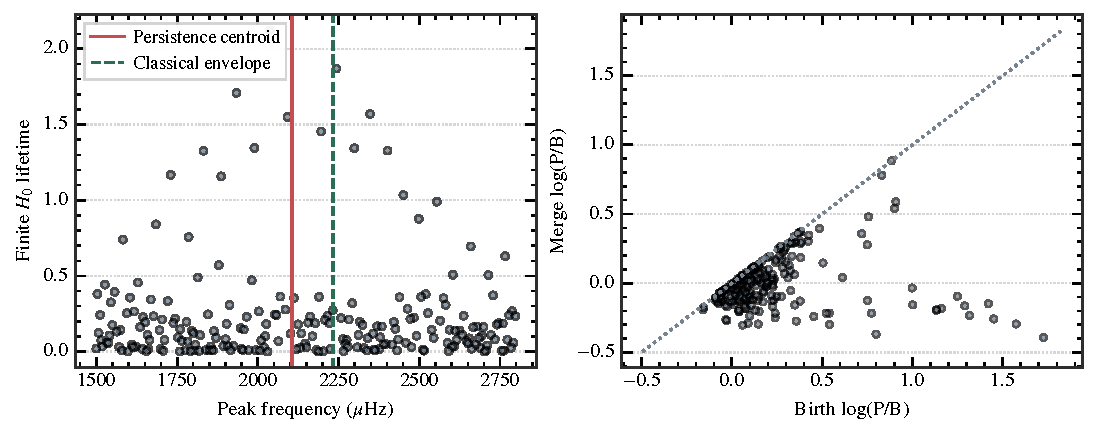
\includegraphics[width=\textwidth]{04_localized_persistence.pdf}
\caption{Finite peak lifetimes and the localized birth--merge diagram.
Essential classes are kept in JSON but excluded from these numeric plots.}\end{figure}
\begin{figure}[p]\centering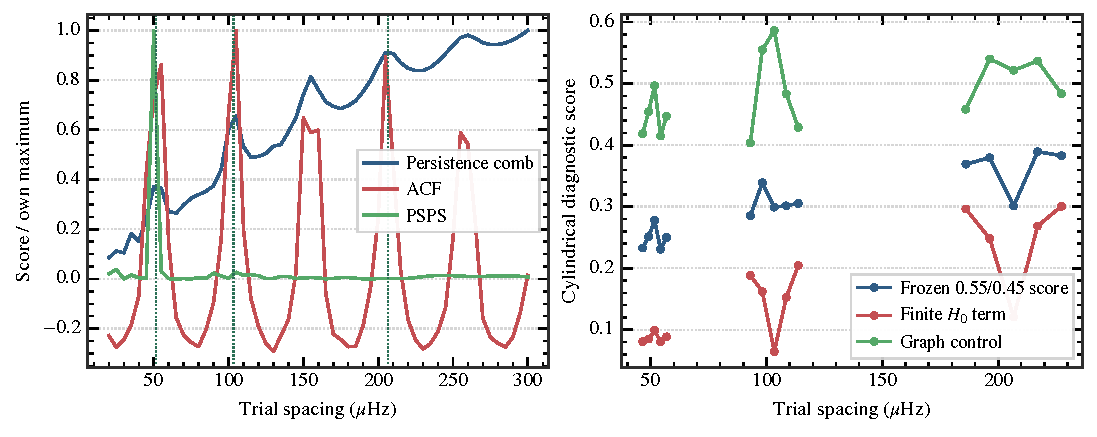
\includegraphics[width=\textwidth]{05_spacing_aliases.pdf}
\caption{Spectral and cylindrical scans retain boundary, half, nominal and
double alternatives. Score selection is not calibrated estimator utility.}\end{figure}
\begin{figure}[p]\centering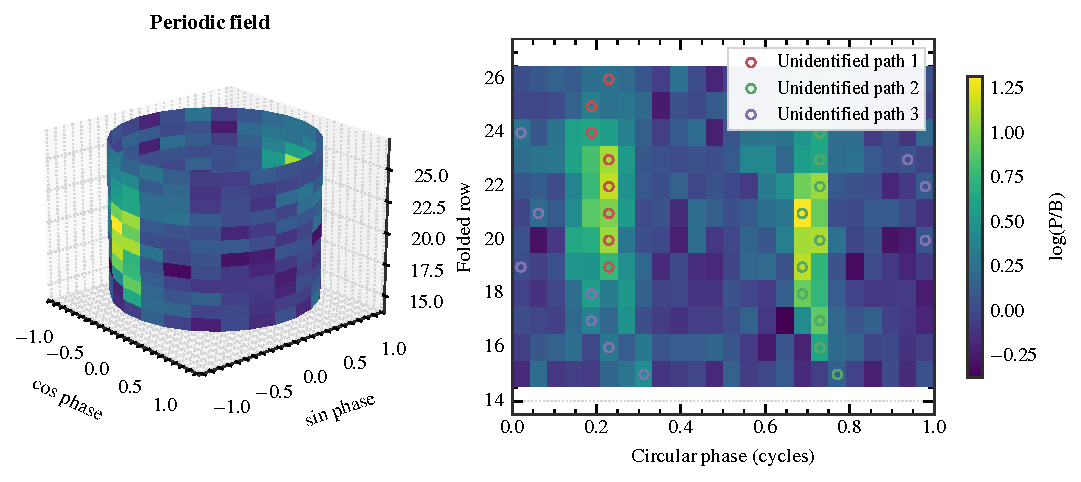
\includegraphics[width=\textwidth]{06_cylinder_ridges.pdf}
\caption{Periodic field and competing unidentified circular graph paths.
No topological frequency ratio is inferred without a defensible degree anchor.}\end{figure}
\begin{figure}[p]\centering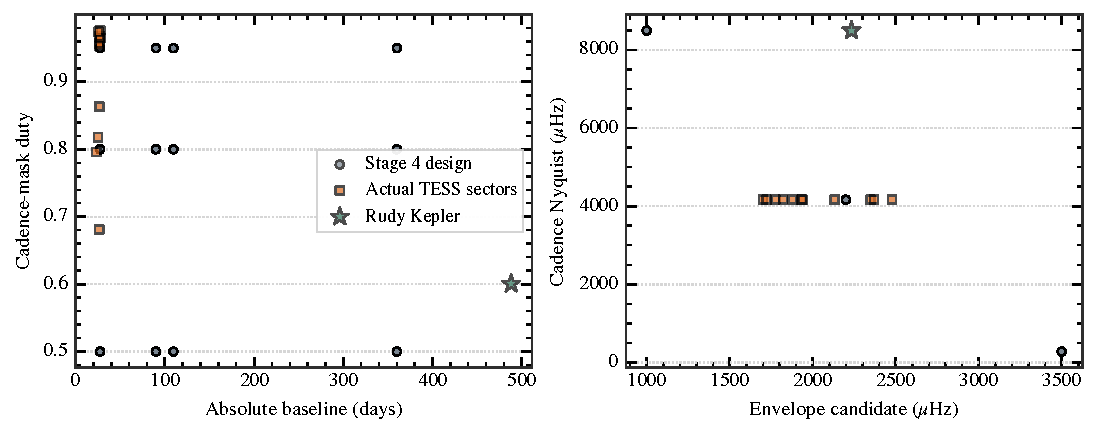
\includegraphics[width=\textwidth]{07_simulation_placement.pdf}
\caption{Observed coordinates against the registered simulation design.
TESS envelope candidates do not imply detections; this is domain context,
not inverse simulation calibration.}\label{fig:placement}\end{figure}
\begin{figure}[p]\centering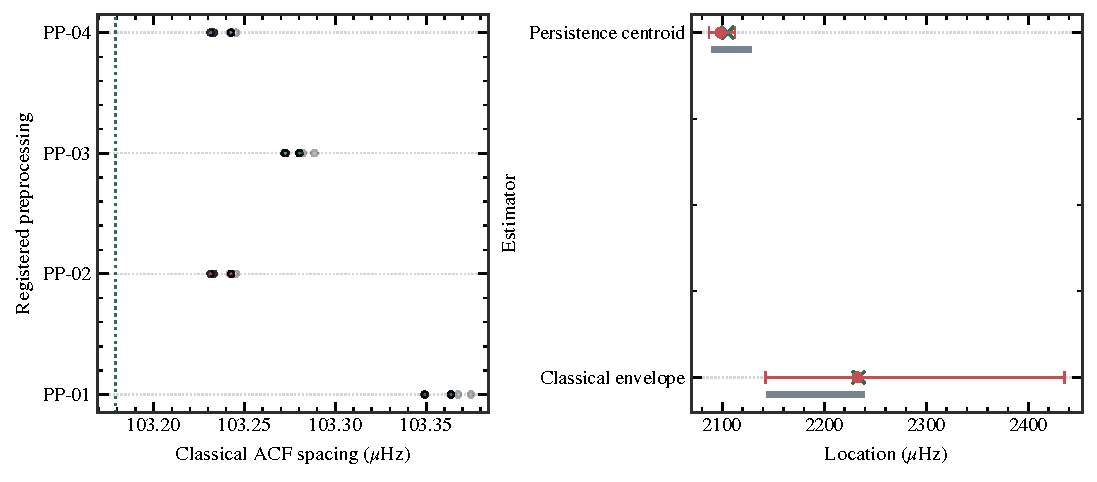
\includegraphics[width=\textwidth]{08_sensitivity_uncertainty.pdf}
\caption{All registered sensitivity diagnostics and distinct uncertainty
targets. Monthly bootstrap bars, pipeline ranges and full-span points are
not combined as independent error budgets.}\end{figure}
\begin{figure}[p]\centering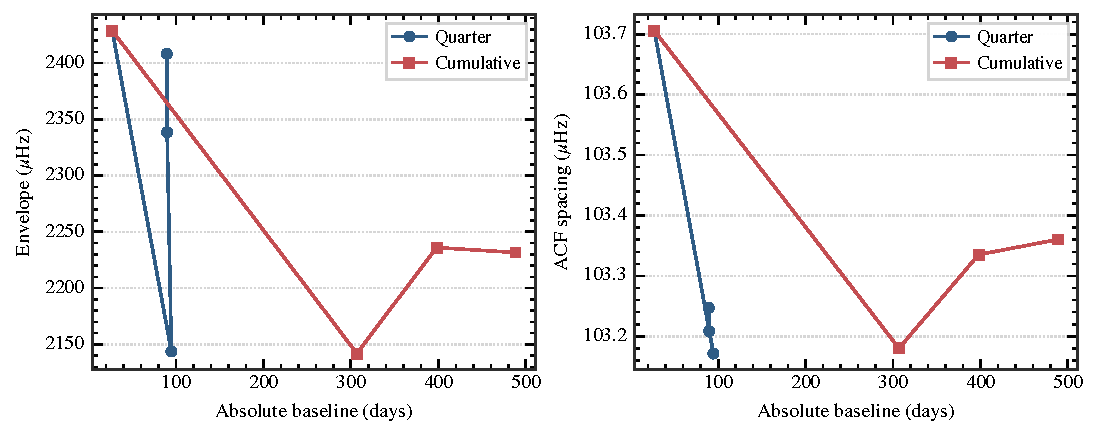
\includegraphics[width=\textwidth]{09_quarter_stability.pdf}
\caption{Quarter and overlapping cumulative-baseline diagnostics with the
primary background held fixed.}\end{figure}
\begin{figure}[p]\centering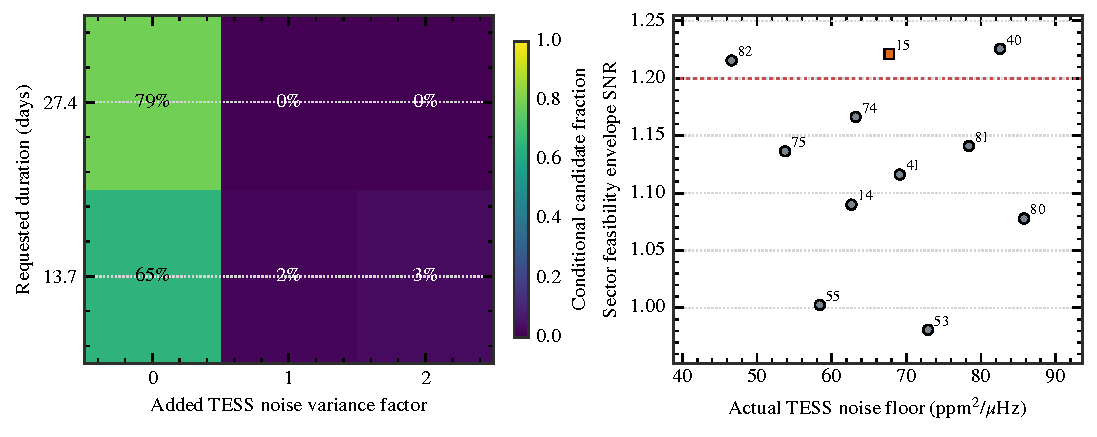
\includegraphics[width=\textwidth]{10_kepler_tess_transfer.pdf}
\caption{Conditional Kepler degradation fractions and actual TESS sector
context. Reused Kepler offsets and real windows are correlated; marginal
candidates are not confirmations.}\label{fig:transfer}\end{figure}
\clearpage
\section*{Frozen claim--evidence ledger}
\paragraph{P1-C01} The public-product capsule and tutorial baseline are reproducible.
\textit{Control:} Lightkurve baseline, frozen payload SHA256. \textit{Limit:} single star and locked pipeline.
\paragraph{P1-C02} Finite path H0 lifetimes are elder-rule prominence, with frequency localization.
\textit{Control:} independent path prominence. \textit{Limit:} no incremental information or novelty claim.
\paragraph{P1-C03} Conditional fitted-background null results are reported with full search maxima and Holm correction.
\textit{Control:} window matched stationary Gaussian background, ACF, PSPS, graph. \textit{Limit:} background fit uncertainty and instrument systematics not calibrated.
\paragraph{P1-C04} Rudy comb and cylindrical scores remain ambiguous diagnostics.
\textit{Control:} ACF, PSPS, conventional echelle, Hough, ridge graph. \textit{Limit:} G8 geometry only no utility or validated coverage.
\paragraph{P1-C05} Monthly resampling, stochastic scatter and registered pipeline ranges target different uncertainties.
\textit{Control:} quarter and cumulative baselines, 72 registered branches. \textit{Limit:} no combined stellar posterior no population inference.
\paragraph{P1-C06} TESS degradation is tested with all real sector windows and actual sectors retained as context.
\textit{Control:} boxcar integration, duration, duty, noise ablations. \textit{Limit:} same Kepler source reused not independent stars or TESS confirmation.
\paragraph{P1-C07} Delay topology is omitted under the registered Stage 7 negative decision.
\textit{Control:} PSD preserving phase and IAAFT surrogates, classical features. \textit{Limit:} no new Rudy phase claim.
\paragraph{P1-C08} Published identified modes support overlays and formula audits only.
\textit{Control:} Lund2017 modes and ratios. \textit{Limit:} no blind degree inference or topological r01 r10.

\clearpage
\bibliographystyle{plainnat}
\bibliography{references}
\end{document}
